\subsubsection{Ecuanimidad SchedLottery con compensation tickets}

SchedLottery fue testeado exhaustivamente y al utilizar el sistema de compensation tickets se comporta de forma esperada. Entre toda la experimentación
decidimos quedarnos con un par de muestras que exhiben aspectos relevantes de su comportamiento.

La siguiente figura muestra un experimento corrido sobre un scheduler con lote de 5 tareas, en donde 1 es bloqueante y las otras consumen constantemente CPU. 
El quantum del mismo es de 4 ticks, por lo que luego de las primeras corridas de cada una tendríamos: 

tarea bloqueante: 4 tickets. Resto de las tareas: 1 ticket. Cantidad de tickets totales en circulación: 8. 

Por lo tanto, lo esperable es que cada 8 sorteos en donde participen las 5 tareas (tengamos en cuenta que cuando una tarea se bloquea una cantidad de clocks $\neq \ 0$ no 
participa en el próximo sorteo), 4 sean ganadas por la tarea bloqueante, y el resto de las tareas gane una única vez.

\begin{figure}[!h]
	\begin{center}
		  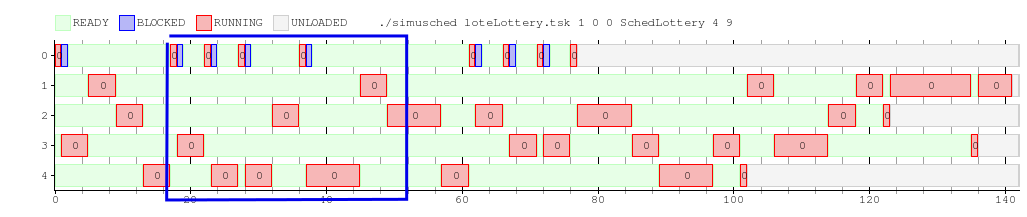
\includegraphics[scale=0.5]{Graficos/intervalo_8.png}
		  \caption{Comportamiento de SchedLottery para 5 tareas: 1 bloqueantes y 4 tareas CPU }
		  \label{fig:contra1}
	\end{center}
\end{figure}
\FloatBarrier

Efectivamente, utilizamos esta figura para mostrar que nuestras hipótesis se confirmaron (el mismo experimento fue corrido repetidas veces arrojando resultados similares).
Si consideramos los sorteos en donde participan las 5 tareas, en el intervalo de tiempo encerrado por el rectángulo azul, observamos como la tarea bloqueante sale
ganadora en 4 de las 8 ocasiones. La tarea 2 gana en 2 ocasiones. La tarea 4 y la 1 ganan en una ocasión (lo esperable), mientras que la tarea 3 no sale sorteada ninguna vez.
